

%-------------------------------------------------------------------------------
% Dokumenten Klasse
\documentclass[
	final,
	a4paper,
	oneside,
	parskip=full,
	headings=standardclasses,
	headings=big,
	pointednumbers
]{scrartcl}

%-------------------------------------------------------------------------------
% Packete nutzen
\usepackage{ngerman,palatino,setspace}
\usepackage[T1]{fontenc}
\usepackage[utf8]{inputenc}
\usepackage[left=35mm,right=35mm,top=25mm,bottom=25mm]{geometry}
\usepackage{amsmath}
\usepackage{mathtools}
\usepackage{tikz}


\usetikzlibrary{automata, positioning, arrows}

%-------------------------------------------------------------------------------
% Dokument
\begin{document}
    
    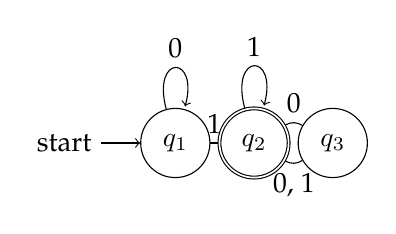
\begin{tikzpicture}
        \node[state, initial] (q1) {$q_1$};
        \node[state, accepting, right of=q1] (q2) {$q_2$};
        \node[state, right of=q2] (q3) {$q_3$};
        \draw (q1) edge[loop above] node{0} (q1)
        (q1) edge[above] node{1} (q2)
        (q2) edge[loop above] node{1} (q2)
        (q2) edge[bend left, above] node{0} (q3)
        (q3) edge[bend left, below] node{0, 1} (q2);
    \end{tikzpicture}

    
\end{document}
